\documentclass[border=2mm, tikz]{standalone}
\usetikzlibrary{arrows.meta, positioning, shadows}

    \begin{document}
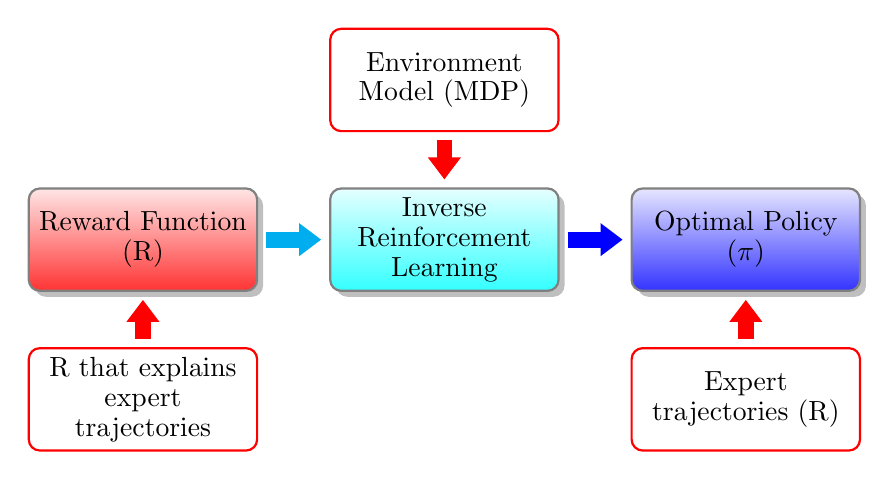
\begin{tikzpicture}[
    node distance = 7mm and 9mm,
    MN/.style args = {#1/#2}{
                    draw=#1,% line color
                   top color=#2!10,
                    bottom color=#2!80,
                    rounded corners, thick,
                    text width=27mm, minimum height=13mm, inner sep=1mm, 
                    align=flush center},
    line/.style = {line width=2mm,
                    draw=#1,%line color
                    -{Triangle[length=2.8mm,width=4mm,fill=#1]},
                    shorten >=1mm, shorten <=1mm},
    ds/.style = {drop shadow}]
%---
\linespread{0.9}
% bottom
\node (n1) [MN=red/white]                   {R that explains expert trajectories};
% middle
\node (n2) [MN=gray/red, ds,above=of n1]    {Reward Function (R)};
\node (n3) [MN=gray/cyan,ds,right=of n2]    {Inverse Reinforcement Learning};
\node (n4) [MN=gray/blue,ds,right=of n3]    {Optimal Policy ($\pi$)};
% bottom
\node (n5) [MN=red/white,below=of n4]       {Expert trajectories (R)};
% top
\node (n6) [MN=red/white,above=of n3]       {Environment Model (MDP)};
% lines
\draw[line=red]     (n6) edge (n3)
                    (n1) edge (n2)  (n5) to (n4);
\draw[line=cyan]    (n2) edge (n3);
\draw[line=blue]    (n3) edge (n4);
\end{tikzpicture}
    \end{document}
